% Copyright 2019 the authors. All rights reserved.

\documentclass[twocolumn]{aastex62}

\usepackage[T1]{fontenc}
\usepackage{amsmath}
% \usepackage{float}

% typography
\renewcommand{\floatpagefraction}{.9}
\setlength{\parindent}{1.\baselineskip}
\newcommand{\acronym}[1]{{\small{#1}}}
\newcommand{\package}[1]{\textsl{#1}}
\newcommand{\gaia}{\textsl{Gaia}}
\newcommand{\pans}{\textsl{Pan-STARRS}}
\newcommand{\DR}{\acronym{DR2}}
\newcommand{\tractor}{\textsl{The Tractor}}
\newcommand{\msun}{\textrm{M}_\odot}
\newcommand{\kpc}{\textrm{kpc}}
\newcommand{\kms}{\ensuremath{\textrm{km}~\textrm{s}^{-1}}}
\newcommand{\bs}[1]{\boldsymbol{#1}}
\newcommand{\masyr}{\ensuremath{\textrm{mas}~\textrm{yr}^{-1}}}
\newcommand{\feh}{\ensuremath{[\textrm{Fe} / \textrm{H}]}}

% Maths
\newcommand{\given}{\,|\,}
\newcommand{\dd}{\mathrm{d}}
\newcommand{\transpose}[1]{{#1}^{\!\mathsf{T}}}
\newcommand{\inverse}[1]{{#1}^{-1}}
\newcommand{\argmin}{\operatornamewithlimits{argmin}}
\newcommand{\argmax}{\operatornamewithlimits{argmax}}
\newcommand{\mean}[1]{\left< #1 \right>}
\renewcommand{\vec}[1]{\bs{#1}}
\newcommand{\mat}[1]{\mathbf{#1}}


\newcommand{\sectionname}{Section}
\newcommand{\equationname}{Equation}
\renewcommand{\tablename}{Table}
\usepackage{upgreek}

\newcommand{\todo}[1]{{\color{red} TODO: #1}}
\newcommand{\ab}[1]{{\color{teal} AB: #1}}
\newcommand{\sa}[1]{{\color{magenta} SP: #1}}
\newcommand{\changes}[1]{{\textbf{#1}}}

% aastex parameters
% \received{not yet; THIS IS A DRAFT}
%\revised{not yet}
%\accepted{not yet}
% % Adds "Submitted to " the arguement.
% \submitjournal{ApJ}
\shorttitle{pal~5's biggest fan}
\shortauthors{bonaca et al.}

%@arxiver{}

\begin{document}\sloppy\sloppypar\raggedbottom\frenchspacing % trust me

\title{Variations in the width, density, and direction of the Palomar~5 tidal tails}

\author[0000-0002-7846-9787]{Ana~Bonaca}
\affiliation{Center for Astrophysics | Harvard \& Smithsonian, Cambridge, MA 02138, USA}
\email{ana.bonaca@cfa.harvard.edu}
\correspondingauthor{Ana Bonaca}

\author[0000-0003-0256-5446]{Sarah~Pearson}
\affiliation{Flatiron Institute, Center for Computational Astrophysics, NY 10010, USA}

\author[0000-0003-0872-7098]{Adrian~M.~Price-Whelan}
\affiliation{Department of Astrophysical Sciences, Princeton University, Princeton, NJ 08544, USA}

\author{others}

\begin{abstract}\noindent % trust me
Stars that escape globular clusters form tidal tails that are predominantly shaped by the global distribution of mass in the Galaxy, but also preserve a historical record of small-scale perturbations.
Using deep $grz$ photometry from DECaLS, we present highly probable members of the tidal tails associated with the disrupting globular cluster Palomar~5.
These data yield the cleanest view of a stellar stream beyond $\sim20\,\rm kpc$ and reveal: (1) a wide, low surface-brightness extension of the leading tail, (2) significant density variations along the stream, and (3) sharp changes in the direction of the trailing tail.
In the fiducial Milky Way model, a rotating bar perturbs the Palomar~5 tails and can produce stream similar width and density profiles to those observed.
However, the deviations of the stream track in this simple model are significantly smaller than those observed in the Palomar~5 trailing tail, so future kinematic observations may identify an additional source of perturbation. \sa{Think this former sentence is slightly confusing as it's saying the models cannot reproduce the observed wiggle, but that future observations will help.}
These discoveries open up the possibility of measuring the population of perturbers in the Milky Way, including dark-matter subhalos, with an ensamble of stellar streams and deep photometry alone.
\end{abstract}

\keywords{Galaxy: halo --- dark matter ---
          Galaxy: kinematics and dynamics}

\section{Introduction}
\label{sec:intro}

Direct N-body simulations of globular clusters in a static galaxy predict that the clusters continually lose stars through evaporation and tidal stripping \citep[e.g.,][]{Baumgardt:2003}.
Stars escape the cluster with a small relative velocity, and thus form thin, kinematically cold streams \citep[e.g.,][]{Combes:1999}.
As a result, globular cluster streams are excellent tracers of the underlying tidal field, and under the assumption of a static potential, they constrain the enclosed mass within their current location \citep{Bonaca:2018}.
Nearby stellar streams have already been used to measure the mass and shape of the Milky Way halo \citep[e.g.,][]{Koposov:2010, Kupper:2015, Bovy:2016}.

However, streams are long-lived and witness the host galaxy evolve, including its gradual increase in mass, its rotating bar, and orbiting dark matter subhalos.
When simulated in more realistic environments that feature some of these events, the resulting streams are no longer 
%regular 
thin, coherent structures \citep[e.g.,][]{Bonaca:2014, Ngan:2015, Price-Whelan:2016b}. Recently, \citet{Price-Whelan:2018} detected gaps and off-the-stream features in the GD-1 stellar stream that could be signatures of perturbation \citep{Bonaca:2018b}.
This discovery establishes stellar streams as a cosmological probe of dark matter on small scales.
However, streams can also be affected by baryonic perturbers, such as giant molecular clouds \citep{Amorisco:2016}, the Galatic bar \citep{Pearson:2017}, spiral arms \citep{Banik:2019}, or even naturally develop features in their density profile during cluster disruption \citep[e.g.,][]{Kupper:2008, Just:2009}. Additionally, stream debris can spread out rapidly in phase space if their progenitors are evolving on non-regular orbits \citep[e.g.,][]{Pearson:2015, Fardal:2015, Price-Whelan:2016}.
To measure the abundance of dark-matter subhalos from stream perturbations, we need to confirm the origin of stream perturbations first.

In this paper, we reassess tidal tails of the Palomar~5 (Pal~5) globular cluster \citep{Odenkirchen:2001, Rockosi:2002}.
The Pal~5 stream features density variations not reproduced in a static model of the Milky Way, but neither their significance nor their origin have been established \citep{Carlberg:2012, Bernard:2016, Ibata:2016, Erkal:2017}.
Arguably, Pal~5 provides the best opportunity for disentangling different mechanisms that shape the stream as it has a surviving progenitor. Such an endeavor, however, requires a robust map of the entire tidal debris.
Pal~5 is located too far ($d = 23$ kpc: \citealt{Dotter:2011}) to enable efficient membership selection based on \gaia\ proper motions, while accurate mapping using the existing photometry is limited because the catalogs are either wide, but shallow \citep{Bernard:2016}, or deep, but narrow \citep{Ibata:2016}.
To confidently identify Pal~5 members over a wide area, we use deep, wide-field photometry from the DECam Legacy Survey (\S\ref{sec:data}).
In \S\ref{sec:densitymodel} we use the updated map of Pal~5 to quantify how the stream track, its width and density vary along the stream.
We then explore how these properties change across Pal~5 models simulated in a range of Galactic potentials (\S\ref{sec:sim_results}) and conclude with a discussion of perturbers that jointly could have caused the observed Pal~5 features (\S\ref{sec:discussion}).


\section{Data}
\label{sec:data}

\begin{figure*}
\begin{center}
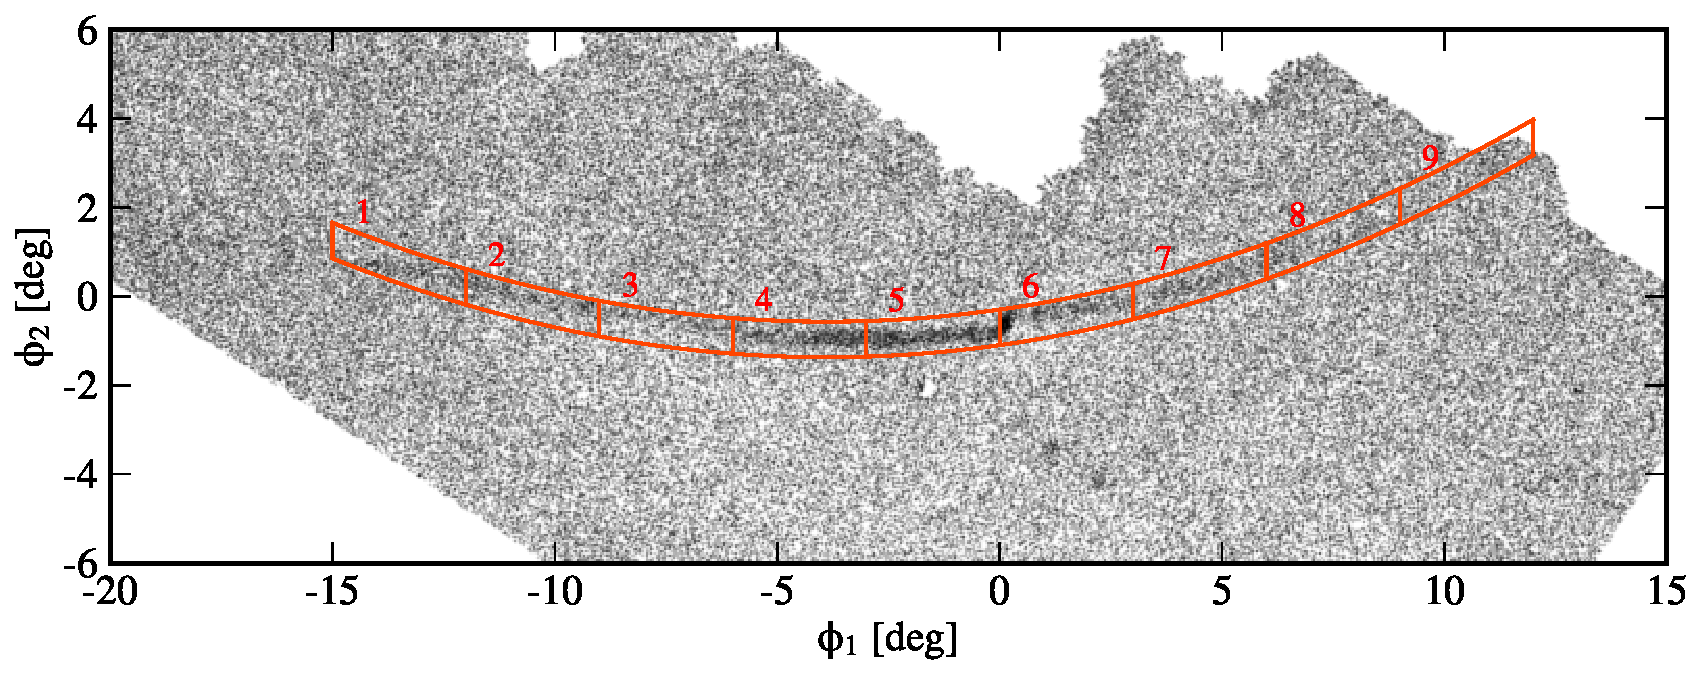
\includegraphics[width=0.83\textwidth]{fig1_a_map.pdf}
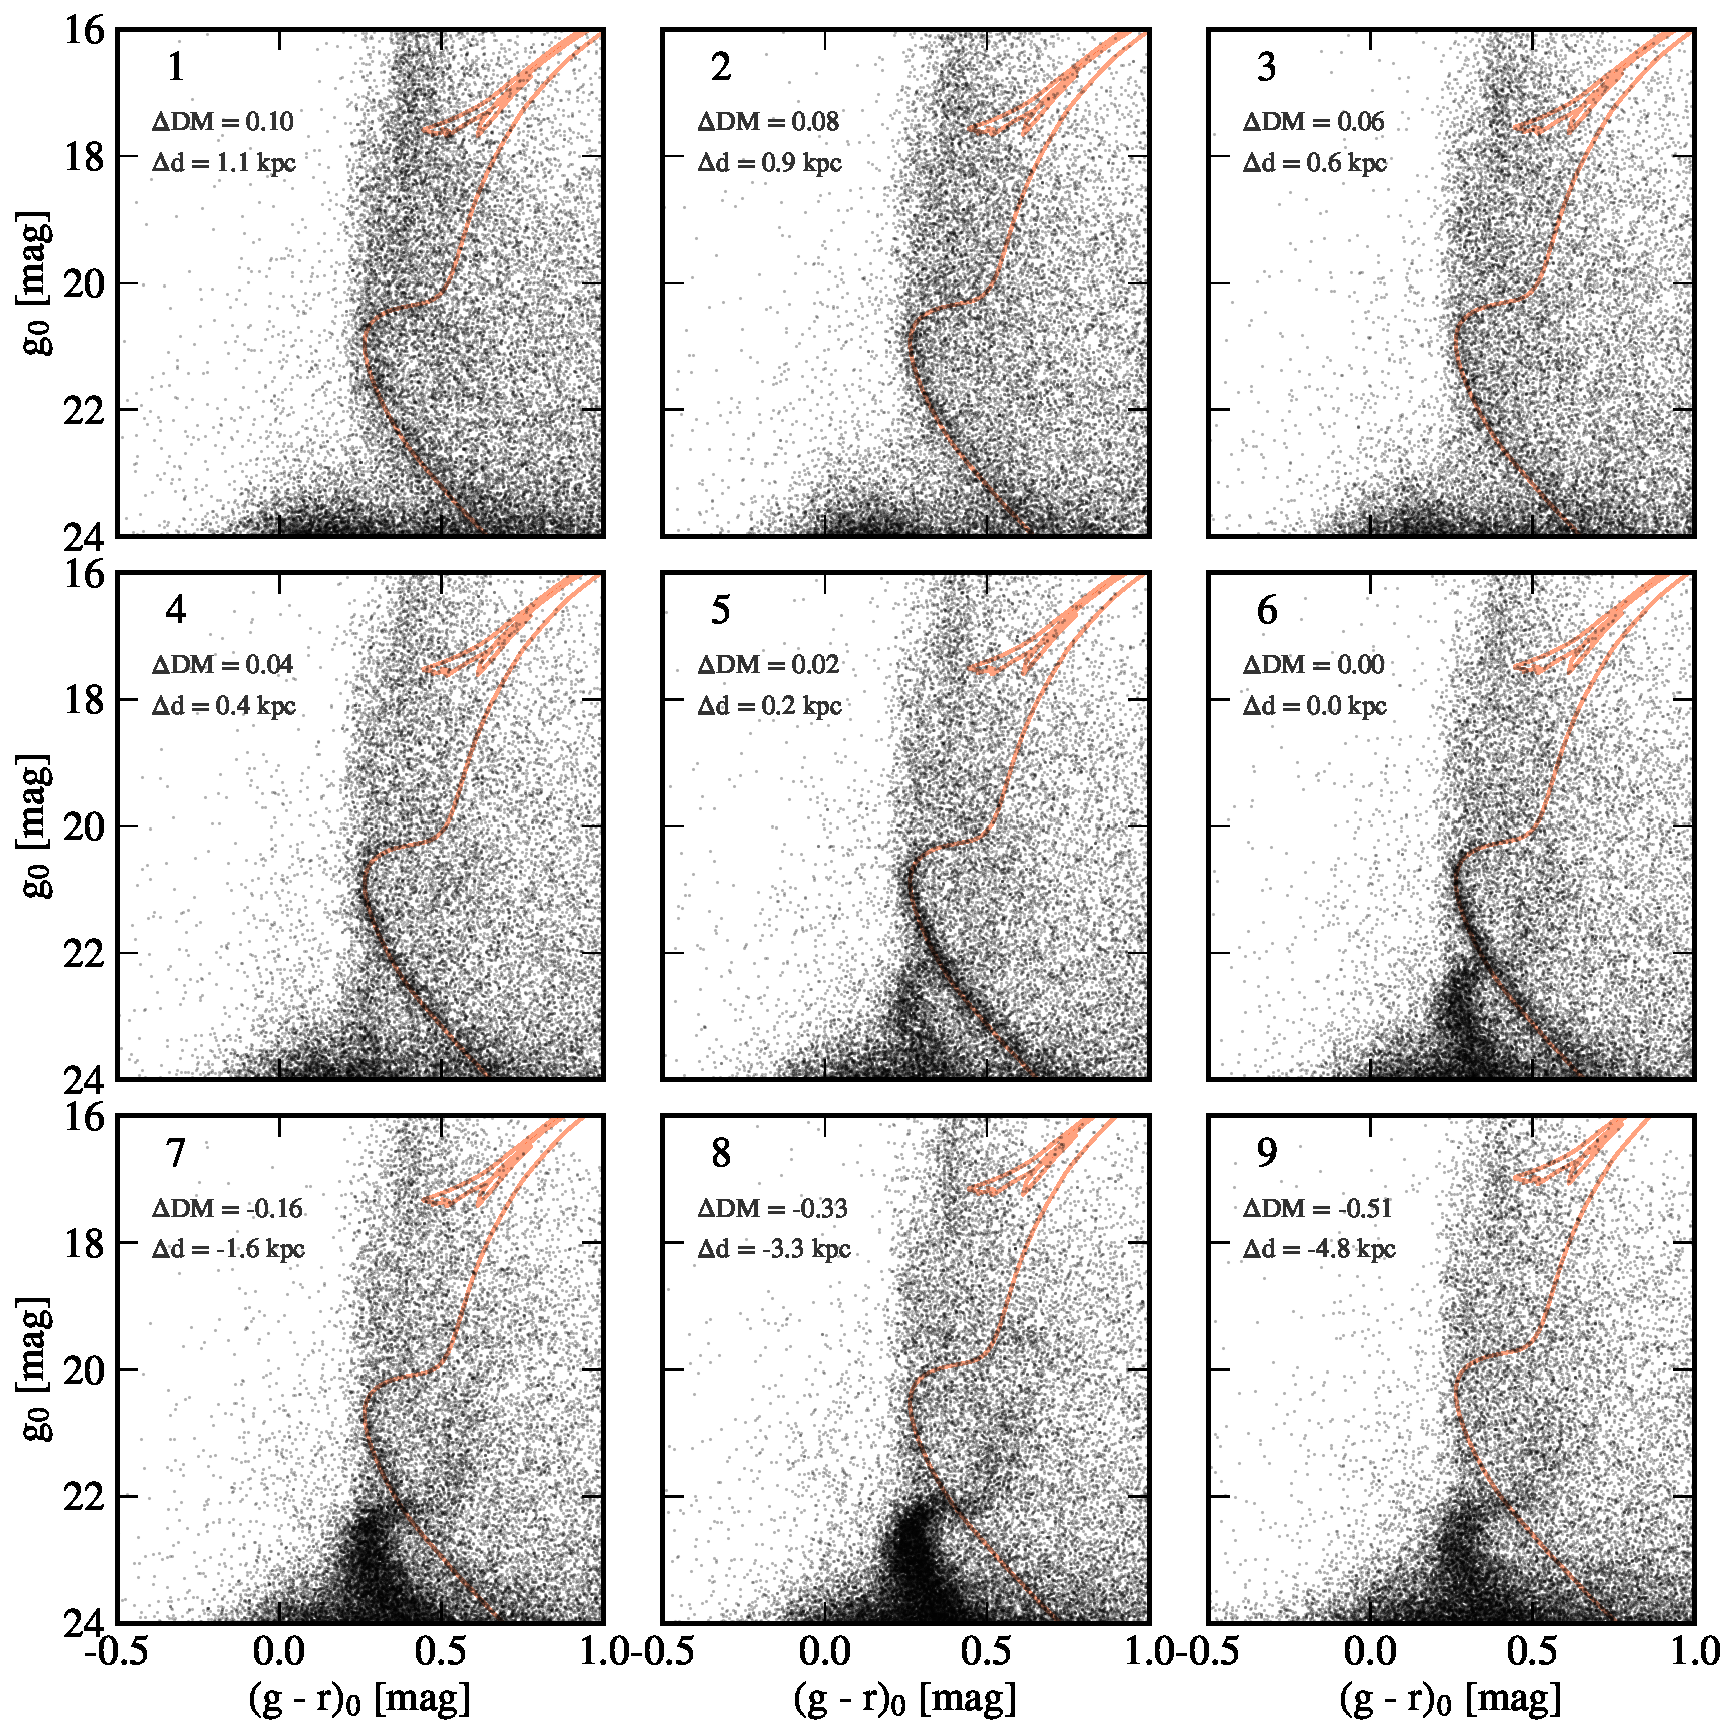
\includegraphics[width=0.83\textwidth]{fig1_b_cmds.pdf}
\end{center}
\caption{
(Top) The Legacy Surveys detection of the Palomar 5 globular cluster in a coordinate system aligned with its tidal tails.
(Bottom) Color-magnitude diagrams of $\approx0.8\times3$\,deg windows along the tails.
The regions are labeled in the top left of each panel, and their sky locations are marked in the top panel.
A stellar population consistent with Pal~5 is evident in every region, although its prominence varies between the fields.
There is a distance gradient along the stream, with the end of the trailing tail ($\phi_1\sim-15^\circ$) being the most distant, and end of the leading tail ($\phi_1\sim10^\circ$) the closest.
The fiducial Pal~5 isochrone is offset in every panel so that it matches the location of the main sequence, and the difference in distance modulus from the fiducial Pal~5 value is indicated in the top left.
}
\label{fig:cmds}
\end{figure*}

We study the Palomar~5 system in the photometric catalog of DECam Legacy Survey \citep[DECaLS, part of the DESI Legacy Imaging Surveys,][]{dey2019}.
The survey was designed to provide deep $grz$ imaging at high galactic latitudes, with the targeted $5\,\sigma$ depth of $g=24$, $r=23.4$, and $z=22.5$.
In addition to data obtained as a part of the survey, DECaLS also includes imaging from publicly available DECam data in the survey footprint.
We conducted a targeted survey of Pal~5 whose data products are now a part of DECaLS (NOAO Proposal ID nos. 2014A-0321, PI: Geha; 2014A-0611, PI: Munoz; 2015A-0620, PI: Bonaca).
The median (minimum) $5\,\sigma$ PSF depth in the Pal~5 region is $g=25.6(25.3)$, $r=25.1(24.8)$, $z=24.1(23.4)$, which makes DECaLS the deepest and largest-area survey of Pal~5.

To select likely Pal~5 stars, we first queried the DECaLS catalog for point sources.
The catalog was constructed using \tractor\ forward-modeling code for source extraction\footnote{\url{https://github.com/dstndstn/tractor}} and a source was classified as \texttt{`PSF'} if the PSF model was preferred to the round exponential model used to represent galaxies\footnote{\url{https://github.com/legacysurvey/legacypipe}}.
We removed spurious sources by requiring \texttt{allmask\_g==0}, \texttt{allmask\_r==0} and \texttt{brightstarinblob==0}.
With this clean stellar catalog, we identified stars on Pal~5's main sequence in the dereddened color-magnitude diagram \citep{Schlegel:1998}.
Specifically, we selected stars following an 11.5\,Gyr MIST isochrone with $\rm [Fe/H] = -1.3$ \citep{Choi:2016} between $20<g<23.7$.

In the top panel of Figure~\ref{fig:cmds} we present the sky distribution of likely Pal~5 main sequence stars.
The $(\phi_1,\phi_2)$ coordinate frame is oriented along the great circle that best-fits the Pal~5 stream, while keeping the cluster at the origin and its motion in the direction of positive $\phi_1$ \citep{gala}.
There is a distance gradient along the Pal~5 stream \citep{Ibata:2016}, so to increase its contrast against the field Milky Way stars, we applied the isochrone selection at two distances: 23\,kpc for $\phi_1<=0^\circ$ and 19\,kpc for $\phi_1>0^\circ$.
With our map, Pal~5 is continuously detected between $\phi_1=-15^\circ$ and $7^\circ$ for the first time.

The color-magnitude diagrams (CMDs) of stars in the Pal~5 stream are shown in the bottom of Figure~\ref{fig:cmds}.
Each panel contains stars from a $3^\circ$ long and $0.8^\circ$ wide area marked in the top of Figure~\ref{fig:cmds}.
The Pal~5 main-sequence turn-off at $g\sim20.5$ stands out in all fields, but the depth to which the main sequence is detected varies from $g\sim24$ close to the cluster to $g\sim22$ in the leading tail.
The non-uniform detection depth is partly due to variable photometric depth (the coverage is shallower in the leading tail), and partly due to contamination from the Sagittarius stellar stream (main-sequence turn-off at $g\sim22$ for $\phi_1\gtrsim-5^\circ$) and faint galaxies ($g\gtrsim23$).
Despite these challenges, the Pal~5 main-sequence is evident even in field~9 ($9^\circ<\phi_1<12^\circ$), beyond the apparent leading tail truncation at $\phi_1\sim7^\circ$.
This indicates that Pal~5 tails may be longer than previously thought.

To improve our selection of Pal~5 members, we first employ the $z$-band to distinguish between faint stars and galaxies more efficiently.
In DECam filters, the $g-z$ color of stars bluer than $g-r\lesssim1.2$ is approximately linear with the $g-r$ color \citep[e.g.,][]{dey2019}.
We adopted the stellar locus of $(g-z)_0 = 1.7\times(g-r)_0 -0.17$.
On the other hand, galaxies span a wider distribution of redder $g-z$ colors at a fixed $g-r$ color.
To exclude faint galaxies, we restrict to sources within 0.1\,mag of the stellar locus.
We limit the sample to sources with $g<23$ to reduce inhomogeneities due to the shallow $z$-band coverage.

To further refine the Pal~5 membership, we next perform the isochrone selection that varies the distance along the stream.
We start by approximating the distance to the nine segments of the Pal~5 stream indicated in Figure~\ref{fig:cmds} from the locations of their main-sequence turn-offs.
The adopted distance modulus is indicated in CMD panels at the bottom of Figure~\ref{fig:cmds}, and the corresponding isochrone is shown in orange.
We perform the updated isochrone selection in $2^\circ$ bins of $\phi_1$ by interpolating the location of the main-sequence selection box between these distance estimates.
With the improved star--galaxy separation and a selection that accounts for the distance gradient along the stream, Pal~5 tails are prominent between $\rm R.A.\sim223^\circ$ and $\sim245^\circ$ (Figure~\ref{fig:map}).

\begin{figure*}
\begin{center}
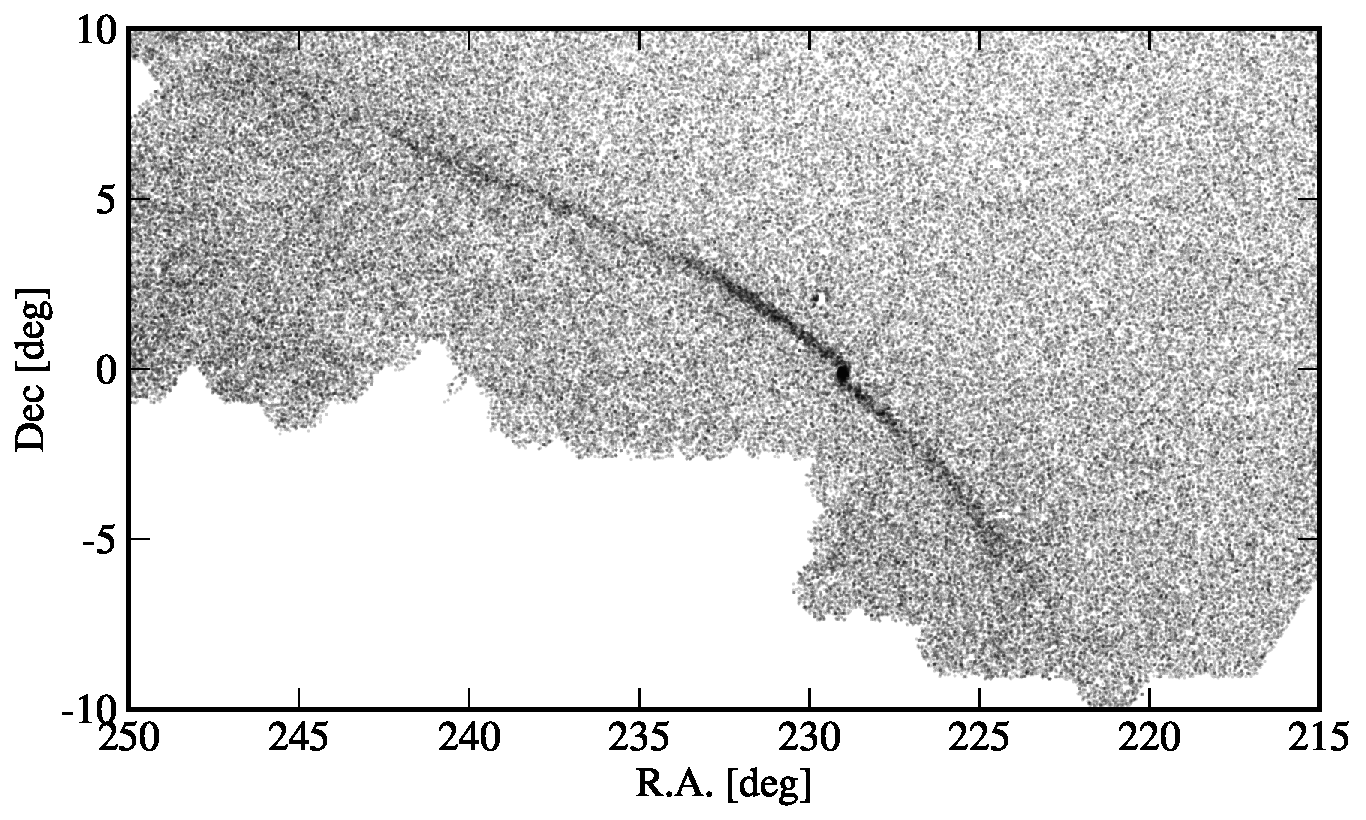
\includegraphics[width=0.85\textwidth]{fig2_map.pdf}
\end{center}
\caption{
The optimized Legacy Surveys detection of the Palomar 5 system reveals: (1) an extremely wide, low surface-brightness extension of the leading tail beyond $\rm Dec<-5^\circ$, (2) prominent underdensities at $\rm R.A.\approx 227^\circ$ and $235^\circ$, and (3) sharp changes in the direction of the stream track at $\rm R.A.\approx 226^\circ$ and $233^\circ$.
These features may be evidence of Pal~5's perturbed dynamical history.
}
\label{fig:map}
\end{figure*}

The DECaLS map of Pal~5 reveals qualitatively new features in the stream.
First, the leading tail extends to $\rm Dec\sim-7^\circ$, beyond the previously detected edge at $\rm Dec\sim -5^\circ$ \citep{Bernard:2016}.
This newly detected extension of the leading tail is very wide ($\sigma\sim 0.25^\circ$) and in stark contrast with the trailing tail at the same distance from the cluster ($\sigma\sim 0.1^\circ$).
Next, there are significant variations in the stellar density along the stream.
At a fixed distance from the cluster, the trailing tail is denser than the leading tail.
Furthermore, both tails feature a prominent gap in the stellar density, located at $\rm R.A.\approx 227^\circ$ and $235^\circ$ for the leading and trailing tail, respectively.
Finally, the stream track sharply changes direction at $\rm R.A.\approx 226^\circ$ and $233^\circ$.

\section{Stream density modeling}
\label{sec:densitymodel}
% adrn: feel free to move this text / or rename section - I just put it here for now to keep it self-contained

We quantify the variations along the Pal~5 stream and measure the stream track, width, and surface density using a constrained Gaussian Mixture Model (GMM) to represent both the stream itself and the background stellar density \citep[our model is similar to, but more flexible than, past work that use GMMs to model streams][]{Erkal:2017, Koposov:2019}.
In detail, our model for the stream surface density consists of a set of $K$, 2D Gaussians---``nodes''---that are equally spaced in the Pal~5 coordinate system longitude, $\phi_1$, with an interval $\Delta$.
The $\phi_1$ locations of each node are fixed, but the $K$ $\phi_2$ locations are included as independent parameters in the model along with each node amplitude $\alpha_k$.
Each node has two width parameters: $h_k$, which defines the along-stream standard-deviation of each node, and $w_k$, which defines the standard-deviation in the perpendicular direction; We fix $h_k = \Delta$ to ensure some overlap between the nodes.
We set the rotation of each Gaussian such that the $h_k$ direction is parallel to the local tangent of the stream track---that is, for a given node $k$ at location $\bs{\mu}_k = (\phi_{1,k}, \phi_{2,k})$, we find the local tangent (using $\bs{\mu}_{k+1} - \bs{\mu}_k$) and construct the rotation matrix $\mat{R}$ to go from the Gaussian node axes to this tangent-aligned coordinate system such that the covariance matrix of each node is given by $\mat{C}_k = \mat{R}_k \, \mat{C}'_k \, \transpose{\mat{R}}_k$, where
\begin{equation}
    \mat{C}'_k =
    \begin{pmatrix}
        h_k^2 & 0 \\
        0 & w_k^2
    \end{pmatrix} \quad .
\end{equation}

The total surface density for this stream model at any location $\bs{x}$ is given by
\begin{equation}
    \rho(\bs{x}) = \sum_k^K \alpha_k \, \mathcal{N}(\bs{x} \given \bs{\mu}_k, \mat{C}_k)
\end{equation}
where $\mathcal{N}(\bs{\mu}, \mat{C})$ represents the multivariate (2D) normal distribution with mean $\bs{\mu}$ and covariance $\mat{C}$.
This model has $3 K$ free parameters associated with the nodes ($\alpha_k$, $\phi_{2, k}$, and $w_k$) which are all allowed to vary independently (that is, unlike the models in \cite{Erkal:2017} and \cite{Koposov:2019}, the node properties are not tied together by a spline or other function).

The background stellar density in this region of the sky does not vary substantially over the field (see, e.g., Figure~\ref{fig:map}), but displays some gradients with sky position that cannot be represented by a purely uniform background.
We therefore also include a flexible background model into our model for the total stellar surface density of this field that we simultaneously infer with the stream density model parameters.
For the background density, we use a constant plus a constrained GMM in which $J$, 2D, circular Gaussian nodes are fixed to a 2D grid of locations over the field, and we fit for the amplitudes of each background Gaussian node, $\alpha_j$.
In more detail, we set up a 2D, rectangular grid over the given sky field with node spacing $\Delta_{\textrm{bg}} = XX^\circ$ at locations $\bs{\mu}_j$ and fixed (circular) standard deviations $h_{\textrm{bg}} = w_{\textrm{bg}} = \Delta_{\textrm{bg}}$.
We only include the amplitudes of each background Gaussian node as free parameters, which, along with the constant value, adds an additional $1+J$ parameters to the total model.

To compare and fit this model to the data, we use this model to predict the stellar number counts in a pixelized histogram representation of the map shown in Figure~\ref{fig:map}; We set the pixel size of to $0.2^\circ$.
We use a Poisson likelihood to compare the predicted counts (from the density model described above) to the pixelized map of Pal~5.
We use a binary-valued 2D selection function (constructed by finding all pixels with $\leq 2$ stars) to mask the model in regions that are not observed.
We implement this stellar surface density model in the \texttt{stan} \citep{stan} probabilistic programming language, which, through automatic differentiation, provides derivatives of the model likelihood with respect to all model parameters that aide in optimization or sampling over this high-dimensional model.
After some experimentation, we set the stream node spacing $\Delta = XX^\circ$.
We initialize the stream node locations by setting the node coordinates by eye, but the node latitude locations, $\phi_{2, k}$, are allowed to move within $\pm 1^\circ$ of each initialized position.
We find the best-fit parameters by optimizing the log-likelihood using the built-in BFGS optimizer \citep{Press:2007}.

\todo{adrn: fill the XX's in the above section}

Figure~\ref{fig:density-model} shows ...


\begin{figure}
% \centerline{\includegraphics[width=\columnwidth]{Placeholder.pdf}}
\caption{One column with three rows showing: 1) data. 2) 2d density model. 3) Residual. Adrian is working on this on the cluster now. 
}
\label{fig:density-model}
\end{figure}



\section{Simulations}
\label{sec:sim}
To explore the mechanism leading the the observed morphology of the stream (i.e. the length asymmetry between the leading and trailing arm, as well as the gap in the trailing arm, and the widening of the leading arm), we run a suite of Pal~5 simulations.
In particular, we investigate whether Pal~5's wide leading arm can be explained due to chaotic regions in the potential, or whether an interaction with the Galactic bar can explain the asymmetric stream width. 
In Section \ref{sec:potential}, we describe the potentials we use to simulate the evolution of Pal~5, and in Section \ref{sec:modeling} we describe our simulation setup.
We show the results of our analyses in Section \ref{sec:sim_results}.

\subsection{Potential}
\label{sec:potential}
\sa{To save word counts, I could just refer to other papers for the BFE representation? Let me know what you think.}
We simulate the evolution of Pal~5 in two classes of three-component Galactic potentials:

\begin{itemize}
\item[1.] {\bf Static potentials}: we use the \texttt{MWPotential2014} \citep{Bovy:2015} consisting of a Miyamoto-Nagai disk (\citealt{Miyamoto:1975}), a bulge modeled as an exponentially cut off, power-law density profile, and an axisymmetric NFW dark matter halo (\citealt{Navarro:1996}).
We vary the flattening of the NFW halo ($q_z = 0.94$ and $q_z = 0.5$) to investigate Pal~5's morphology on a regular as well as chaotic orbit (see Section \ref{sec:modeling}).

\item[2.] {\bf  Barred potentials}: we use the same disk and halo as in the {\small MWPotential2014}, but include a Galactic bar instead of a bulge.
Following \citet{wang:2012}, we compute the bar potential as a basis-function expansion (BFE) representation of a triaxial, exponential density profile:
\begin{align}
    \rho_{\rm bar} &= \rho_0 [{\rm exp} (-r^2_1/2) + r_2^{-1.85} {\rm exp}(-r_2) ]\\
    r_1 &= \left[\left((x/x_0)^2 + (y/y_0)^2\right)^2 +( z/z_0)^4\right]^{1/4}\\
    r_2 &= \left[\frac{q^2(x^2 + y^2) + z^2)}{z_0^2}\right]^{1/2}
\end{align}
where the scale lengths are $x_0$ = 1.49 kpc, $y_0$ = 0.58 kpc, $z_0$ = 0.4 kpc, and q = 0.6. We include terms up to $n=6$, $l=6$ in the ``self-consistent field" BFE formalism\footnote{\citet{Banik:2019} found that using higher order terms (e.g. n=9, l = 19) for the basis function expansion yields a better representation of the density of the bar. Our simulations of Pal~5, however, show that this difference does not much change the morphology or kinematics of the Pal~5 stream.}.
We explore barred models with pattern speeds of $\Omega_b$ = ($30 - 60$) $\kms$ kpc$^{-1}$ in increments of 0.5 $\kms$ kpc$^{-1}$, and  we test bar masses of M$_{\rm bar} = 5 \times 10^{9}$ $\msun$ and M$_{\rm bar} = 1 \times 10^{10}$ $\msun$ (\citealt{Portail:2017}).
Additionally, we fix the present day angular offset from the Galactic x-axis in the direction of rotation to $\alpha = 27\deg$.
\end{itemize}

Note that \citet{wang:2012} constructed a bar with a pattern speed of $\Omega_b$ =  60 $\kms$ kpc$^{-1}$, which has a co-rotation radius, $r_{\rm CR} = 3.7$ kpc.
%This is the radius at which the circular frequency ($\Omega_0$) is equal to the spin of the bar ($\Omega_b$) including the mass of the total potential.
In this paper, however, we explore a range of pattern speeds, which will lead to different co-rotation radii for different pattern speeds (faster bars have co-rotation at smaller radii and vice versa).
As bars are not expected to extend much beyond their co-rotation radius (\citealt{binney:2008}), we therefore adjust the physical scaling of the bar when we vary the pattern speed. %In \citet{wang:2012}, the scale-radius, $r_s$, assumed in the BFE, is  $r_s = 1.1$ kpc.
In particular, we compute the co-rotation radius, $r_{\rm CR},$ for the mass profiles of the static potential for any given pattern speed, $\Omega_b$.
We then scale the bar model for a given pattern speed, $\Omega_b$, by:
\begin{equation}\label{eq:scale}
r_{s, \Omega_b}  = r_{{\rm CR}, \Omega_b}/r_{{\rm CR, Wang 2012}}
\end{equation}
If the scaling in Equation \ref{eq:scale} is not included (e.g. in %\citealt{price:2016b},
\citealt{Pearson:2017}, \citealt{Erkal:2017}, \citealt{Banik:2019}), the bar will have a too strong quadrupole for faster pattern speeds, and a too weak bar quadrupole for  slower pattern speeds.

% In Figure \ref{fig:vcirc}, we show the circular velocity as a function of radius for the barred, three-component Galactic potential with $\Omega_b$ = ($25 - 65$) $\kms$ kpc$^{-1}$. The red lines correspond to the potentials with a bar mass of $M_{\rm bar} = 5 \times 10^{9}$ $\msun$, and the blue lines correspond to potentials with a bar mass of  $M_{\rm bar} = 1 \times 10^{10}$ $\msun$.
%
% \begin{figure}
% \centerline{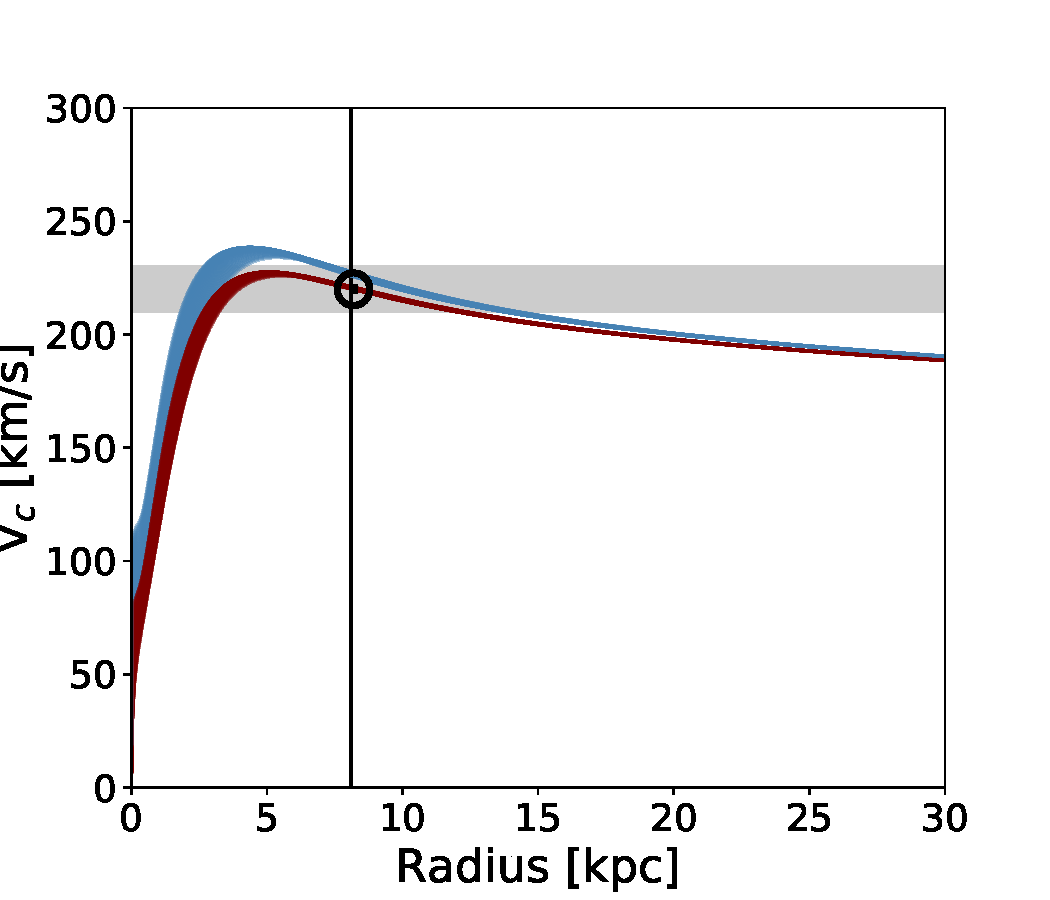
\includegraphics[width=\columnwidth]{v_circ_nlm919.pdf}}
% \caption{\todo{Probably include static potential as well, and show the different components of the potentials }}
% \label{fig:vcirc}
% \end{figure}


\subsection{Stream modeling}
\label{sec:modeling}
\sa{Att. APW: describe stream track fitting...}
To simulate the evolution of Pal~5 in a given potential, we first transform Pal~5's observed 6D phase space coordinates into a Galactocentric frame by assuming $v_{lsr} = (11.1, 24.0, 7.25) ~\kms$,  $v_{circ} = 220  ~\kms$ and a distance from the Sun to the Galactic center of 8.1 kpc.
At present day, the Pal~5 globular cluster is located at: RA = 229.0264 deg, Dec = $-0.1368$ deg, at a distance of $d$ = 22.50 kpc. Its moving with a radial velocity of $v_r = -56.2 \kms$, and has proper motions of pm$_{RA,cosdec}= -2.21$ mas yr$^{-1}$ and pm$_{Dec} = -2.23$ mas yr$^{-1}$. \sa{Check references for these values - I took them from gala.coordinates.pal5$_c$ in notebook}
%RA = 229.018 deg, Dec = - 0.24 deg, at a distance of $d$ = 22.9 kpc. Its moving with a radial velocity of $v_r = -58.7 \kms$, and has proper motions of pm$_{RA,cosdec}= -2.296$ mas yr$^{-1}$ and pm$_{Dec} = -2.257$ mas yr$^{-1}$.
We integrate the cluster backwards in time for 3 Gyr in steps of 0.5 Myr (see potentials in Section \ref{sec:potential}).
Subsequently, we simulate the forward evolution of Pal~5 using the ``particle-spray'' stream generating method developed by \citet{Fardal:2015} and implemented in the \package{gala} package (\citealt{gala}), such that the cluster ends at its present day position at $t = 0$. We release two particles through each of the two Lagrange points from the progenitor every time step (i.e. 2 particles every 0.5 Myr for 3 Gyr). We account for the self-gravity of the Pal~5 cluster by including the cluster as a Plummer profile with size = 4 pc and a of mass 14,404 M$_{\odot}$. 

To investigate Pal~5's evolution on a regular orbit, we first run a ``particle-spray'' simulations setting $q_z = 0.94$ (\citealt{Bovy:2016}).
Subsequently, we run the same simulation setting $q_z = 0.5$ to induce a chaotic orbit.
Additionally, we simulate the evolution of Pal~5's stream in barred potentials, where we first integrating the orbit backwards for 3 Gyr, and then create mock streams as described above.
We vary the pattern speed of the bar, while updating its physical scaling (see Section \ref{sec:potential}, % and Figure \ref{fig:vcirc}).
and we repeat this exercise using bar masses of both M$_{\rm bar} = 5 \times 10^{9}$ $\msun$ and M$_{\rm bar} = 1 \times 10^{10}$ $\msun$.

\sa{Will stste that we didn't actually fit for the track, density or width in our simulations} 

\subsection{Simulation results}
\label{sec:sim_results}
\sa{In progres..}\\
In Figure \ref{fig:sims}, we present the morphology of the simulated Pal~5 streams in various potentials.
The first two rows show Pal~5 evolved in a static potential with two different flattenings ($q_z = 0.94$ and $q_z = 0.5$).
In the last two rows, we highlight two particular simulations of mock streams evolved in time-dependent barred potentials. Before selecting these two examples, we visually inspected the morphology, track and width of the simulated streams in the barred potentials. 
%with M$_{\rm bar} = 5\times 10^9$ M$_{\odot}$ and $5\times 10^9$ M$_{\odot}$ as well as pattern speeds in the range of $\Omega_b = 30-60 ~\kms$ kpc$^{-1}$ in increments of $0.5~\kms$ kpc$^{-1}$.
%In Figure \ref{fig:sims}, we highlight two particular mock-streams as 
The stream evolved in the Bar1 example (third panel) demonstrates a scenario where the leading arm has been abruptly truncated in its density as compared to the trailing arm which is denser at further distances from the cluster. The mock stream evolved in Bar2. on the other hand, produced a leading arm which is widened and a trailing stream which has been perturbed by the bar as well. 

In Figure \ref{fig:model-sim-compare}, we present the track (left), width (middle) and density (right) from our 2D density model of the data (solid black line) as well as the 2D density model of each of our simulated streams shown in Figure \ref{fig:sims} (colored lines). %From the morphology alone (Figure \ref{fig:sims}), 
The regular stream reproduce the widening of the leading arm which is clearly seen in the 2D density model of the data. 
%This is seen in width (Figure \ref{fig:model-sim-compare}, left) as well. 
While the chaotic orbit produces a stream which is widened, this effect is symmetric and occurs for both the leading and trailing arm (see xx line in Figure \ref{fig:model-sim-compare}). Thus, this simulation does reproduce the asymmetry in length nor density of the leading and trailing arm. \sa{I'll finish this section for the barred sims once we have plot.}

While our exploration of mock-streams evolved in various potentials can individually reproduce some of the observed features presented in Figure \ref{fig:map}, none of the presented simulations reproduce all gaps, the widening of the leading arm, the stream tracks nor density profile simultaneously. Note, however, that we did not individually fit for the stream track, width nor density and our simulations are therefore only meant to demonstrate how various effects can play a role in shaping the Pal~5 stream. 

\begin{figure}
% \centerline{\includegraphics[width=\columnwidth]{Fig4_sims.pdf}}
\caption{Mock-streams of the Pal~5 stream simulated in a static potential on a regular orbit (top panel), in a static potential on a chaotic orbit (second panel), in a time-dependent barred potential with M$_{\rm bar} = 5\times 10^9$ M$_{\odot}$ and $\Omega_b = 38$ $\kms$ kpc$^{-1}$ (third panel), and in a barred potential with M$_{\rm bar} = 1\times 10^{10}$ M$_{\odot}$ and $\Omega_b = 45$ $\kms$ kpc$^{-1}$ (fourth panel). The regular orbit produces a symmetric and thin leading and trailing arm,  whereas the chaotic orbit leads to a symmetric and widened leading and trailing arm (note that we limit the footprint to show  only the extent of thedata presented in the top panel of Figure \ref{fig:cmds}). The stream evolved in the Bar1 potential leads to a truncated leading arm, while the stream evolved in the Bar2 simulation produces a widened leading arm, and also shows signs of asymmetric perturbations to the trailing arm. }
\label{fig:sims}
\end{figure}


% \section{Density model}
% \label{sec:density}
% To compare our data and various Pal~5 simulated streams, we construct density model consisting of a multicomponent Gaussian mixture model. In particular, we are interested in fitting the width and density of our data and simulated stars.
%
% We first transform our simulated Pal~5 data points to the tangent sky plane using a Zeanit (Lambert azimuthal) equal-area projection, such that we can define a Gaussian. We call these coordinates, $X$, $Y$.
%
% We then fit a 3rd order polynomial to the leading and trailing arm separately, in this projected space.
%
% We place K nodes, k, equally in distance along the polynomial fits to the leading and trailing arm.
%
% At each node, k, along the polynomial we find the tangent/parallel unit vector,  $\hat{u}$, and the perpendicular normal unit vector, $\hat{v}$, to the stream.
%
% At each node, k, we define the co-variance matrix, $\tilde{C_k}$:
%
% \begin{equation}
% \tilde{C_k} =
% \begin{pmatrix}
%     h^2 & 0  \\
%     0 & S_k^2  \\
% \end{pmatrix}
% \end{equation}
% where $h$ is bandwidth of the Gaussian components along the polynomial fit and $S_k$ is the  width of the Gaussians in the perpendicular (normal) direction of the stream at any node, k.
%
% We transform it from the space spanned by the $\hat{u}$,  $\hat{v}$ vectors to $X$, $Y$:
% \begin{equation}
% C_k = \rm{R} \tilde{C_k} \rm{R}^T
% \end{equation}
% where
% \begin{equation}
% \rm{R} =
% \begin{pmatrix}
%     \rm{cos} \theta & - \rm{sin} \theta  \\
%     \rm{sin} \theta & \rm{cos} \theta \\
% \end{pmatrix}
% \end{equation}
% and  $\theta$ is the angle between the tangent sky plane and the unit vector, $\hat{u}$.
%
% To compute our density model along the leading at trailing stream, for the K nodes, k, we define ln density  and sum over the K nodes:
% \begin{equation}
% \rm{ln} \sum ( \alpha_k \mathcal{N}\left(\mu_k, C_k\right))
% \end{equation}
% where $\mu_k$ denotes the location of each node, k, along the leading and trailing polynomial fits, respectively, $C_k$ is the covariance matrix, and $\alpha_k$ is the amplitude of the Gaussian (representing density at specific node, k).
%
% We then fit for the perpendicular width, $S_k$, to the stream (polynomial fits) and the amplitude of the Gaussians, $\alpha_k$, which represent the density along the stream.
%
% %Explain background model for data.
%
% We compute the width and density of both or simulated Pal~5 streams and the DECaLS data fitting the above Gaussian mixture model.

\begin{figure}
% \centerline{\includegraphics[width=\columnwidth]{Placeholder.pdf}}
\caption{One row with three panels showing:\\
Track for 2d density model (solid black line) along with inferred track of the simulation points from 2d model (colored lines indicating 4 sims from figure 4). The y axis is deltaphi2 and the x-axis is phi1.\\
Width for 2d density model (solid black line) along with inferred width of the simulation points from 2d model (colored lines indicating 4 sims from figure 4). The y axis is wphi2 and the x-axis is phi1.\\
Density for 2d density model (solid black line) along with inferred density of the simulation points from 2d model (colored lines indicating 4 sims from figure 4). The y axis is rho0,phi1 and the x-axis is phi1.
}
\label{fig:model-sim-compare}
\end{figure}



\section{Discussion}
\label{sec:discussion}
\sa{Do we want to emphasize how streams might all look messed up as we get deeper maps?  }
We presented deep $grz$ photometry of the Palomar~5 tidal tails from the Legacy Surveys catalog that enables the cleanest selection of Pal~5 members to date.
Our flexible, 2D modeling of the debris' spatial distribution yielded unprecedented measurements of the width and density along the tidal tails, and revealed 
%for the first time 
changes in the direction of the trailing tail. \sa{wondering if unprecedented is too strong of a word?}
Our different simulations
%models 
of stellar streams
%that are globally perturbed 
separately capture many of the features observed in Pal~5, including an asymmetry in the length and the width of the leading and trailing tail.
However, these specific simulations fail to reproduce the observed gaps in the stream density and the wiggles of its track.
In this section we discuss perturbing mechanisms that could jointly explain this transformed view of the Pal~5 stream.
% \ab{rephrase as needed once the rest of the analysis is in place}

The striking asymmetry in the length and width of Pal~5's two tidal arms is immediately obvious from Figure~\ref{fig:map}.
\citet{Pearson:2017} showed that the short leading arm, first reported in \citet{Bernard:2016}, may be truncated through a perturbation by the Milky Way's Galactic bar. 
%SP removed the word "repeated" as the leading arm can by truncated on just one pericentric passage.
This scenario predicts that the bar sweeps tidal debris from the leading arm to a much wider area. 
%The specific model presented in \citet{Pearson:2017} predicts the presence of low-surface brightness debris beyond $\rm Dec\lesssim-5^\circ$ (previous detection limit). %SP: this debris was at dec -30 deg. 
Deep, wide-field DECaLS photometry enabled us to trace the leading tail as it fans out to $\rm Dec\sim-7^\circ$, while the color-magnitude diagram implies Pal~5 debris has been spread out to even lower surface-brightness level between $-7^\circ\gtrsim\rm Dec\gtrsim-10^\circ$. In Section \ref{sec:sim_results}, we showed that this low surface-brightness feature can indeed be induced if Pal~5 has been perturbed by the bar. 
%SP: I removed the word "confirming".

The bar is a prominent perturber that affects objects within 5\,kpc from the Galactic center \citep[e.g., the Ophiuchus stream,][]{Price-Whelan:2016b, Hattori:2016} to the Solar circle and beyond \citep[e.g., local phase-space overdensities][]{Hunt:2018, Monari:2019}.
Recent progress investigating the Galactic bar, is converging on a pattern speed close to $\Omega_b \sim 40 ~\kms$ kpc$^{-1}$ \citep[e.g.,][]{Clarke:2019, Sanders:2019, Bovy:2019}, however the bar properties remain somewhat uncertain. A combination of future deeper imaging along Pal~5's leading tail and a quantitative analysis of its width and density could provide important constraints on the mass and pattern speed of the Galactic bar. Careful modeling of interactions with the Milky Way's spiral arms and molecular clouds, however, would be necessary as well (\citealt{Banik:2019}, \citealt{Amorisco:2016}. 
% SP added last sentence above and changed transition below: we have to account for all perturbers at once (molecular clouds, spiral arms, dm subhalos)

Encounters with a compact perturber can produce a gap in a stellar stream \citep[e.g.,][]{Johnston:2002,Ibata:2002}. As streams are excellent record-keepers of small-scale perturbations, the tidal tails of Pal~5 have long been searched for such density variations.
The findings so far have been conflicting, with the number of gaps reported in Pal~5 ranging from five \citep{Carlberg:2012} to no gaps \citep{Ibata:2016}.
With DECaLS photometry, we confirm the large-scale density variations reported by \citet{Erkal:2017}: the two most prominent underdensities in Pal~5 are a $\sim5^\circ$ gap in the trailing and a $\sim1^\circ$ gap in the leading tail. 
\ab{update gap sizes}
The presence of gaps by itself does not distinguish the nature of the perturber, with dark-matter subhalos and molecular clouds being two plausible alternatives \citep[e.g.,][]{Yoon:2011,Amorisco:2016}.
Based on mass arguments, \citet{Erkal:2017} suggested that the large gap in Pal~5 originates from a dark-matter subhalo encounter, while the small gap may have been produced by a molecular cloud.
In addition to the perturber's mass, details of the gap profile also depend on the time since the encounter and its impact parameter \citep{Erkal:2015}.
Our dataset enables a confident measurement of the gap profile above the Milky Way field contamination \ab{quantify a bit?}, which opens up the possibility of disentangling different encounter parameters.
%SP thinks the sentence below can be omitted. 
%Ultimately, such modeling will determine the nature of Pal~5's small-scale perturbers and measure the abundance of low-mass dark-matter subhalos in the Milky Way halo. 

The depth of the DECaLS catalog also allows for a more confidently determined stream track and reveals its surprising deviations: a global change in Pal~5's curvature $\sim5^\circ$ from the cluster, and $\sim20'$ oscillations, or wiggles, in the trailing tail (Figure~\ref{fig:density-model}).
Neither of these features is reproduced in our simulations, even those that have been perturbed by a rotating bar \ab{confirm this with the new simulations} (\citealt{Erkal:2017} models feature a similar discrepancy). \sa{I think the curvature is actually captured, but not the wiggles, so we should re-phrase.}
Fisher information considerations in a static gravitational potential imply that the stream track encodes the enclosed mass at the current location of the stream \citep{Bonaca:2018}.
The change in the Pal~5's curvature occurs at a nearly symmetric position along the leading and the trailing tail, so this may indicate a sudden change in the enclosed mass inside Pal~5's orbit.
For example, when a stream encounters a massive object, its overall orbit can change and produce a misalignment between the proper motions and the stream track \citep{Erkal:2018, Koposov:2019}.
Measuring the relative angle between the proper-motion vector and the stream track along the Pal~5 tails would therefore test whether it has encountered a massive perturber.
\ab{Does the timing work out with Sgr falling in? Ie, how old is the 10deg chunk of the stream (5deg on either side of the progenitor)?}

Similarly, the small-scale wiggle in the trailing tail may be another signature of an impact, especially as it coincides with a very prominent gap (Figure~\ref{}).
During the encounter, nearby stream stars receive a velocity kick that changes their orbital energies and opens a gap in the stellar stream \citep[e.g.,][]{Erkal:2015b}.
In addition, stream stars affected by the perturber can be displaced from the original stream track \citep{Bonaca:2018b}.
Simultaneous fitting the Pal~5 stream track and its density profile could determine the origin of the trailing tail gap.
Should the encounter scenario be confirmed, track wiggles may put additional constraints on the impact geometry.


%%%%%%%Sp I'd omit the lines below%%%%
%Despite advancing 
%revolutionizing 
%our account of Pal~5's history, the most important implications of our discoveries may be regarding the future studies of stellar streams in general. 
%\sa{I changed "revolutionizing" to "advancing", but I am also not sure we even advances the account Pal~5's history as we didn't find (or attempted to find) a scenario that reproduced all Pal~5 features. }
% Perhaps most importantly, our discoveries bode well for future studies of stellar streams.

As valuable tracers for 3D mapping of matter in galaxies, streams have already provided constraints on the mass of the Large Magellanic Cloud \citep{Erkal:2019} and revealed the presence of a yet unidentified, low-mass object in the Milky Way halo \citep{Bonaca:2018b}.
Both of these studies relied on the kinematic data from the \gaia\ mission for a confident identification of the stream's member stars.
In this work, we have shown that deep photometry alone can be similarly leveraged to cleanly map tidal debris.
Within the Milky Way, this can enable measuring the abundance of low-mass perturbers in the outer halo by studying distant streams that typically reside outside of \gaia's scope \citep[cf.][]{Ibata:2019}.
Streams at greater galactocentric radii are less likely to have been affected by baryonic structures \citep[e.g.,][]{Banik:2019}, so their dynamical models will more directly constrain the nature of dark matter.
Prominent stellar streams have also been discovered outside of the Local Group \citep[e.g.,][]{Martinez-Delgado:2010, Kado-Fong:2018}, while future surveys are primed to find numerous low-mass steams \citep{Pearson:2019}. 
%SP: I removed the word accretion events, as pearson19 discussed GC streams.
Initially, extragalactic streams will be detected almost exclusively photometrically, and our results show that useful information can be extracted from modeling the stream morphology alone. 
% but our results suggest that will still allow precise three-dimensional mapping of their host galaxies, and thus provide a unique test of the $\Lambda$CDM cosmology. 
\sa{I rephrased this last sentence, as we didn't do any potential fitting or 3d mapping in this paper. }





% \subsection{Deeper stream data}
% Do all streams look crazy if we get deeper data?
% Discuss ``stream-fanning", bar, VL2 Bonaca paper.
% 
% \subsection{Other perturbers}
% As Pal~5 is moving prograde with respect to the disk it will be subject to interactions with both the bar (\citealt{Hattori:2016}%, \citealt{price:2016b}
% ), molecular clouds (\citealt{Amorisco:2016}) and possibly spiral arms (\citealt{Banik:2019}). Additionally, dark matter substructure could be interacting with the stream.
% Pal~5 apocentric distance is $\sim 18$ kpc, and the cluster is therefore probing the inner part of the Galatic potential.
% Hence, it might be unlikely that there are many dark matter subhalos in this part of the halo (\citealt{Garrison-Kimmel:2017}).
% However, the GD1 stellar stream orbit probes a similar region of the Galatic potential, and shows evidence of an interaction with a dark substructure (\citealt{Price-Whelan:2018}, \citealt{Bonaca:2018b}) as the data shows a gap and a ``spur" (\citealt{Yoon:2011}).


\acknowledgements{
It is a pleasure to thank... 
This work was performed in part during the Gaia19 workshop and the 2019 Santa Barbara Gaia Sprint (also supported by the Heising-Simons Foundation), both hosted by the Kavli Institute for Theoretical Physics at the University of California, Santa Barbara. The Flatiron Institute is supported by the Simons Foundation. 


% \appendix
% \section{Math for density model}
% We define our likelihood function, $\mathcal{L} $, as:
%
% \begin{equation}
%     \begin{split}
%      \mathcal{L} = P(\{x_n\} \given \{\mu_k\}, \{C_k\}, \{\alpha_k\} ) &=
%             \prod_n \sum_k P(x_n \given \mu_k, C_k, \alpha_k )  \quad
%     \end{split}
% \end{equation}
% where $K$ is the total number of nodes, $\mu_k$ is the mean position of each node, $N$ is the total number of ``data points", $\alpha$ is the amplitude, $x_n$ = $\begin{pmatrix} x\\  y \end{pmatrix}$ is the data points and $P$ is:
% \begin{equation}
%     \begin{split}
%        P(x_n \given \mu_k, C_k, \alpha_k ) = \alpha_k \mathcal{N}(x_n \given \mu_k, C_k)  \quad
%     \end{split}
% \end{equation}
%
% $C_k$ is the covariance matrix in the $X,Y$-space which is the tangent plane sky projection. We transform to $X,Y$-space from the space spanned by the $\hat{u}$,  $\hat{v}$ vectors:
% \begin{equation}
% C_k^{(x,y)} = \rm{R} \tilde{C_k} \rm{R}^{\rm T}
% \end{equation}
% where
% \begin{equation}
% \tilde{C_k}^{(\hat{u},\hat{v})} =
% \begin{pmatrix}
%     {\rm h}^2 & 0  \\
%     0 & S_k^2  \\
% \end{pmatrix}
% \end{equation}
% and where h is bandwidth of the Gaussian components (which we fix) along the polynomial fit, and $S_k$ is the  width of the Gaussians in the perpendicular (normal) direction of the stream at any node, k. R is the rotation matrix from $\hat{u}$,  $\hat{v}$ to $X, Y$-space:
%
% \begin{equation}
% \rm{R} =
% \begin{pmatrix}
%     \rm{cos} \theta & - \rm{sin} \theta  \\
%     \rm{sin} \theta & \rm{cos} \theta \\
% \end{pmatrix}
% \end{equation}
% and  $\theta$ is the angle between the tangent sky plane and the unit vector, $\hat{u}$.
%
% To optimize for the likelihoods, we compute the analytic derivatives of the log likelihoods, ln$\mathcal{L}$:
%  \begin{equation}
%  \begin{split}
%     {\rm ln} \mathcal{L} = \sum_n {\rm ln} \left[\sum_k P(x_n \given \mu_k, C_k, \alpha_k)\right]  \quad
%     \end{split}
% \end{equation}
% hence, we want to compute:
%  \begin{equation}
%  \begin{split}
%     \frac{\partial{\rm ln} \mathcal{L}}{\partial \alpha_k}, \frac{\partial{\rm ln} \mathcal{L}}{\partial \mu_k}, \frac{\partial{\rm ln} \mathcal{L}}{\partial S_k}  \quad
%     \end{split}
% \end{equation}
%
% To do so, we need to use the following:
%  \begin{equation}
%  \begin{split}
%  |C_k^{-1}|^{1/2} = \frac{1}{{\rm h} S_k},
%    \end{split}
% \end{equation}
%
%  \begin{equation}
%  \begin{split}
%   \alpha_K = 1 - \sum_k^{K-1} \alpha_k,
%    \end{split}
% \end{equation}
%
%  \begin{equation}
%  \begin{split}
%  \mathcal{N}(x_n \given \mu_k, C_k) = \frac{1}{2\pi}|C_k^{-1}|^{1/2} {\rm exp}\left[-\frac{1}{2}(x_n - \mu_k)^{\rm T} C_k^{-1} (x_n - \mu_k) \right]  \quad
%    \end{split}
% \end{equation}
%
% We can now compute the partial derivatives of the log likelihoods, $\partial$ln$\mathcal{L}$:
%  \begin{equation}
%  \begin{split}
%     \frac{\partial{\rm ln} \mathcal{L}}{\partial \alpha_k}  = \sum_n \frac{ \mathcal{N}(x_n \given \mu_k, C_k) -  \mathcal{N}(x_n \given \mu_K, C_K)}{\sum_k \alpha_K \mathcal{N}(x_n \given \mu_K, C_K)} \quad
%     \end{split}
% \end{equation}
% \todo{check capital K's above}
% and
%
%  \begin{equation}
%  \begin{split}
% \frac{\partial{\rm ln} \mathcal{L}}{\partial \mu_k} = \sum_n \frac{\alpha_k \mathcal{N}(x_n \given \mu_k, C_k) C_k^{-1} (x_n - \mu_k)}{\sum_k \alpha_K \mathcal{N}(x_n \given \mu_K, C_K)}
%     \end{split}
% \end{equation}
% and
%
%  \begin{equation}
%  \begin{split}
% \frac{\partial{\rm ln} \mathcal{L}}{\partial S_k} = \sum_n \frac{\alpha_k \mathcal{N}(x_n \given \mu_k, C_k)}{\sum_k \alpha_K \mathcal{N}(x_n \given \mu_K, C_K)} \left[ \frac{1}{S_k} \left(\frac{1}{S_k^2} \left( \frac{1}{b_2} {\rm cos \theta} -  \frac{1}{b_1} {\rm sin} \theta \right)^2 - 1\right)\right]
%     \end{split}
% \end{equation}
% where
% $\begin{pmatrix} b_1\\  b_2 \end{pmatrix}= x_n - \mu_k$.
%
% %\begin{equation}
% %    \begin{split}
% %    p(\phi_2 \given \bs{\theta}) &=
% %            \alpha_{\textrm{bg}} \, \mathcal{U}(-10, 5) \\ & \quad +
% %            \alpha_{\textrm{s}, 1} \, \mathcal{N}(\phi_2 \given \mu_{\textrm{s}}, \sigma_{\textrm{s}, 1}) +
% %            \alpha_{\textrm{s}, 2} \, \mathcal{N}(\phi_2 \given \mu_{\textrm{s}}, \sigma_{\textrm{s}, 2}) \\ & \quad +
% %            \alpha_{\textrm{f}} \,
% %                \mathcal{N}(\phi_2 \given \mu_{\textrm{f}}, \sigma_{\textrm{f}})
% %    \end{split}
% %\end{equation}
%
%
% %
% % This work has made use of data from the European Space Agency (ESA) mission {\it
% % Gaia} (\url{https://www.cosmos.esa.int/gaia}), processed by the {\it Gaia} Data
% % Processing and Analysis Consortium (DPAC,
% % \url{https://www.cosmos.esa.int/web/gaia/dpac/consortium}). Funding for the DPAC
% % has been provided by national institutions, in particular the institutions
% % participating in the {\it Gaia} Multilateral Agreement.  This research was
% % started at the NYC Gaia DR2 Workshop at the Center for Computational
% % Astrophysics of the Flatiron Institute in 2018 April.
% %
% % AB acknowledges generous support from the Institute for Theory and Computation
% % at Harvard University.
% % All code used in this work and all results are available at
% % \url{https://github.com/adrn/GD1-DR2}.
% }

\software{
    \package{Astropy} \citep{astropy, astropy:2018},
    \package{dustmaps}\footnote{\url{https://github.com/gregreen/dustmaps}},
    \package{gala} \citep{gala},
    \package{IPython} \citep{ipython},
    \package{matplotlib} \citep{mpl},
    \package{numpy} \citep{numpy},
    \package{scipy} \citep{scipy},
    \package{stan} \citep{stan}
}

\bibliographystyle{aasjournal}
\bibliography{pal5fan}

\end{document}
